%!TEX root = ../main.tex
\section{Dataset}
\label{sec:dataset}
We built our custom dataset and created  definitions for the success of a post in order to
answer the following research questions: \emph{What makes a text successful  among
conspiracy theorists?}, \emph{What are the keywords making a post get the most  attention
from this kind of audience?}.  In this section, we describe how we retrieved posted  text
from conspiracy theorists on Facebook, how we analyzed these posts and define our own 
metric for \emph{impact}.

\subsection{Data Retrieval}
We built our own dataset using posts from Facebook. We gathered these posts using 
CrowdTangle\footnote{https://crowdtangle.com}, ``a public insights tool owned and operated
by Facebook''~\citep{ctshiffmanciting}. While having some limitations this tool lets us 
find posts by specifying keywords. Our goal was to create a dataset containing posts of 
conspiracy theorists. Besides searching posts including a keyword, one can choose between
posts of a Facebook group or posts of a Facebook page. Crowdtangle only supports groups
which are public (i.e. every Facebook  users can read the posts of the group and join it
without an invitation) and have over 2000 members. One can also exclude posts, group names
or page names containing a certain word. We wanted the dataset to contain at least 30,000 posts to be able to used in deep neuronal network as they require more training
data as simpler models. In order to achieve this, two problems had to be tackled. First we
had to choose wisely which keywords to include in our search. Second we needed to find
actual conspiracy theory discussion groups instead of ones posting ironic content. As these
pages and groups share false information, they are a deletion target of Facebook. We
chose a popular video containing wrong information and clearly had conspiracy
theorists as target audience for our search. We then crawled for posts which shared this video.
Using the downloaded list we extracted the groups these posts belonged to. In CrowdTangle we
sorted these groups by their total interaction count in the last month.  Facebook offers
 to react to a post by clicking on an emoji, writing a comment or by sharing the post 
with others. A post  with a lot of
interaction was usually seen by more people and thus was more important. Groups with more
interactions in total are more active and usually had more members than groups with fewer
interactions. Choosing groups with high interaction counts has two advantages. First we
gain more posts for a given time span than from groups with lower interaction counts in
the same time span. Second the posts themselves have usually more individual interactions.
Using this sorted list we handpicked ten groups (a list of names can be found in
Figure~\ref{fig:dataset-group-names}) of which we were sure are groups run by actual
conspiracy theorists and not just sharing conspiracy theories ironically. 

Along with the conspiracy group dataset, we collected a second dataset consisting of
post from Russia Today's Facebook page (rtnews). Russia Today is known for  publishing
false information and conspiracy theories as shown by \citet{yablokov2015conspiracy}. 

\subsection{Dataset description}
\label{subsec:dataset:description}
For both datasets we decided to only include posts which were at least two months old. The
 idea behind this was that as a post gets older it moves down in the timelime of a group
or  page. The further down a post moves the less attention it receives. With posts being
over two months old, the chances are higher that the interaction count will not change
much over time. Naturally there are exceptions: for example an old post could be shared
on a very popular page. Then this  post might see a strong increase in interactions even
if it is older than two months. This is a limitation resulting from our decision. 

Among others we get following features for each post: post type (can be one of \emph{Link},
\emph{Native Video}, \emph{Photo}, \emph{Status}, \emph{Video}, \emph{YouTube}), number of
interactions (\emph{Likes}, \emph{Comments}, \emph{Shares}, \emph{Love}, \emph{Wow},
\emph{Haha}, \emph{Sad}, \emph{Angry}, \emph{Care}), message, link (points to the shared
video or link), image text (for  post type \emph{Image}, Facebook uses
OCR\footnote{optical character recognition} to extract  text which is displayed in the
image), link text, description and total interactions.

\subsection{Data Preprocessing} The preprocessing consisted of two steps. 
\begin{enumerate} 
    \item We removed posts with duplicate content. In our Facebook group dataset this is
more likely  as different members might share the same content more than once. On the other
hand, for
Facebook pages  this is rather unlikely as the rtnews page is run by a single
organization which coordinates all published posts. We considered a post as a duplicate
if the message and image text were equal. For the rtnews set we considered a post
being a duplication if message, link text, image text and description were equal. 
    \item We created our own score variable which we tried to predict later and added it to
each row of the dataset. A detailed description of this variable can be found in a  later
part of this section. 
\end{enumerate}
For rtnews this resulted in a removal of only 1\% of the posts. These posts happened to
have no message,  image text, link text and description at all. At the end we were left
with 57,650 posts. For the group dataset 52\% of the posts were duplications, leaving us
with 33,638 posts. 
\begin{figure}[tb] 
    \centering
    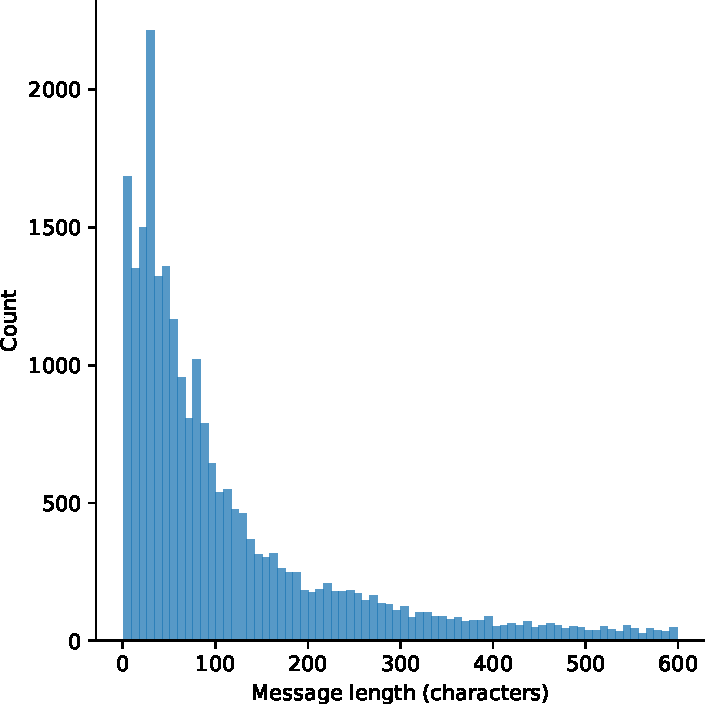
\includegraphics[width=.32\textwidth]{figures/dataset_groups/message_length_dist.pdf}
    \raisebox{-0.7cm}{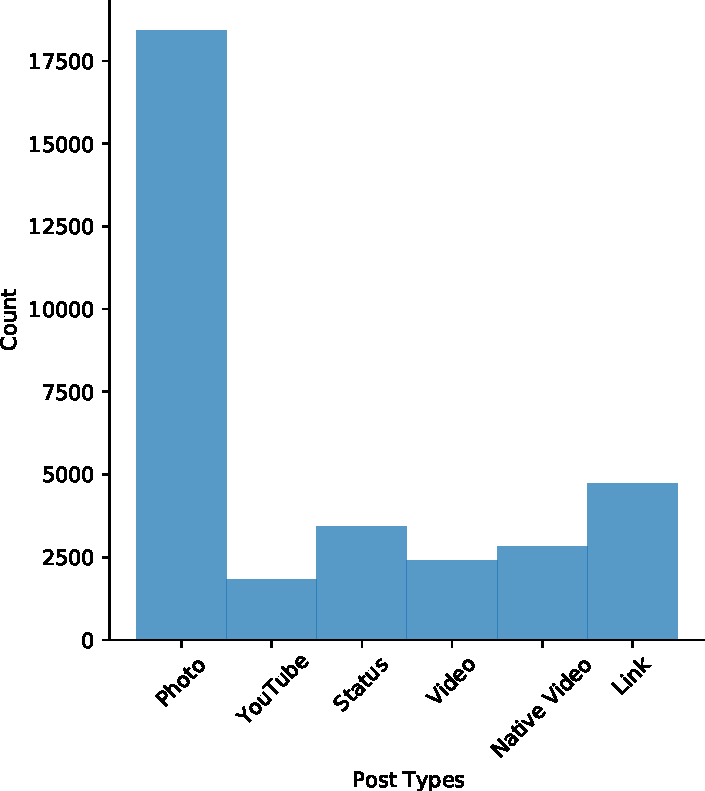
\includegraphics[width=.32\textwidth]{figures/dataset_groups/post_types_dist.pdf}}
    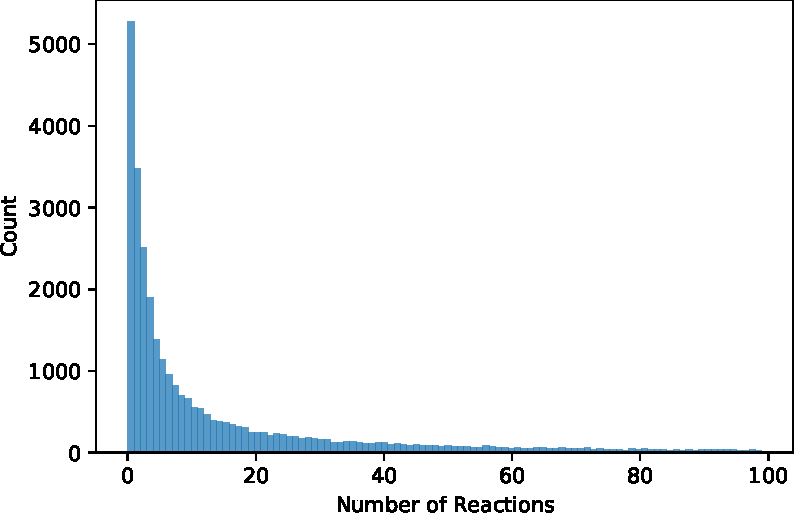
\includegraphics[width=.32\textwidth]{figures/dataset_groups/reactions_dist.pdf}
    \caption{Facebook Conspiracy Theory Group Dataset}
    \label{fig:datasetstats-groups}
\end{figure} 
\begin{figure}[tb] 
    \centering
    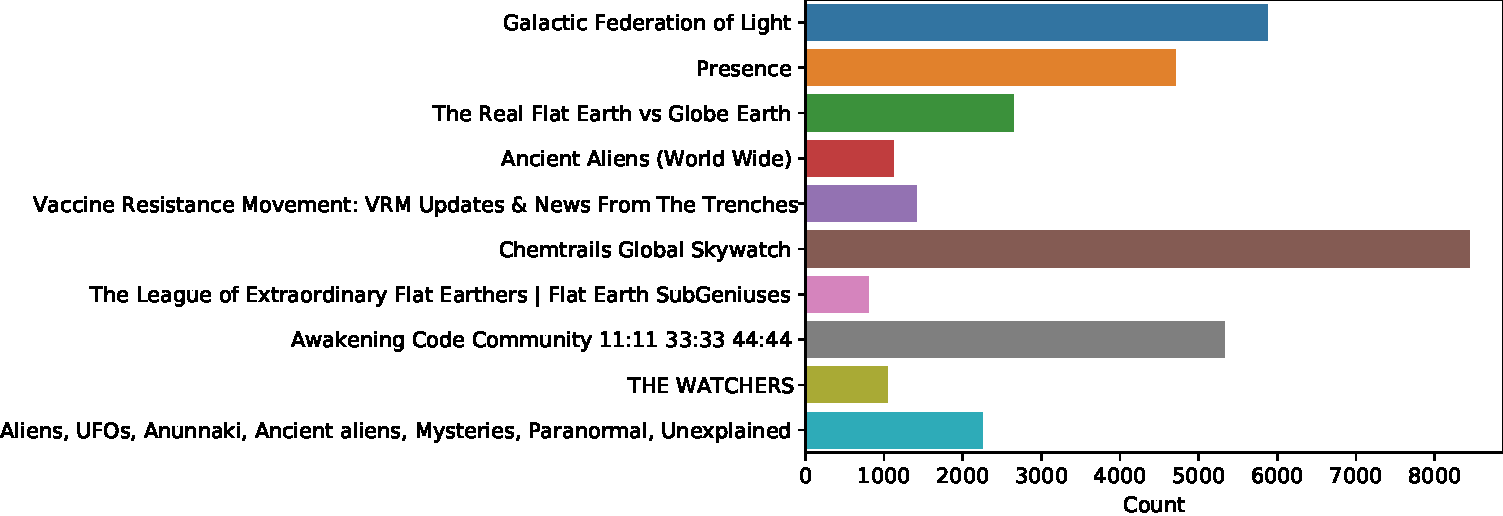
\includegraphics[width=\textwidth]{figures/dataset_groups/group_dist.pdf}
    \caption{Facebook Conspiracy Theory Groups}
    \label{fig:dataset-group-names}
\end{figure}
Figure~\ref{fig:datasetstats-groups} shows the distribution of message length, post type 
and number of reactions for the group dataset. Most messages were below 500 characters and
got less than 20 reactions. As Facebook  already provided us with the text extracted from
images, the high amount of image post  was no issue for us. As mentioned before, we
already removed all duplicate posts. If no text could be  extracted from the image and the
message was the same, the post would have already been removed as part of the preprocessing.
As the number of group members influences the number of reactions, we tried to overcome
the unequal distribution of groups (Figure~\ref{fig:dataset-group-names}) by including the
group's ID as a feature for our models. 
\begin{figure}[tb] 
    \centering
    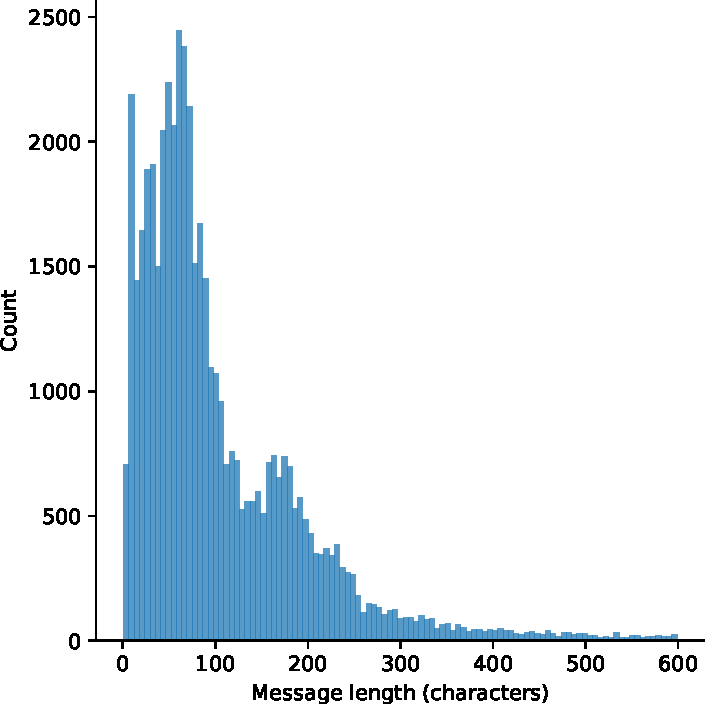
\includegraphics[width=.28\textwidth]{figures/dataset_rtnews/message_length_dist.pdf}
    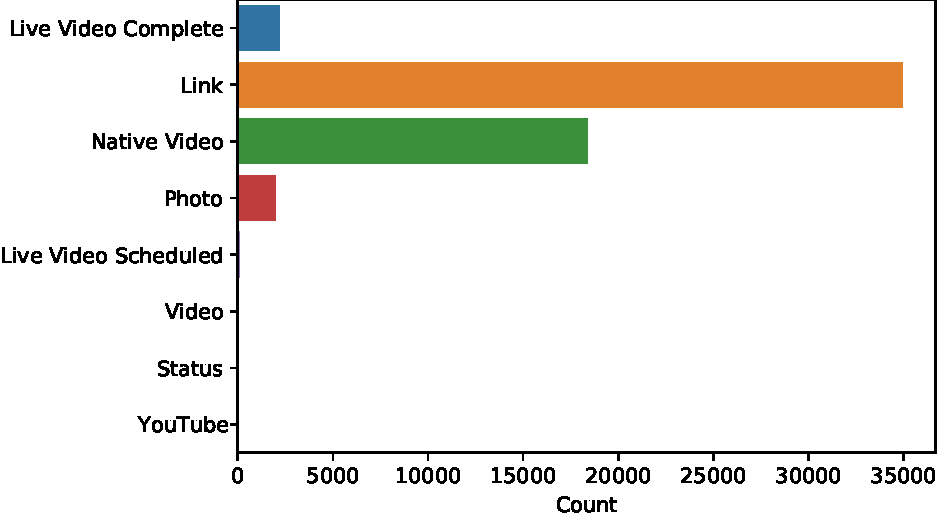
\includegraphics[width=.40\textwidth]{figures/dataset_rtnews/post_types_dist.pdf}
    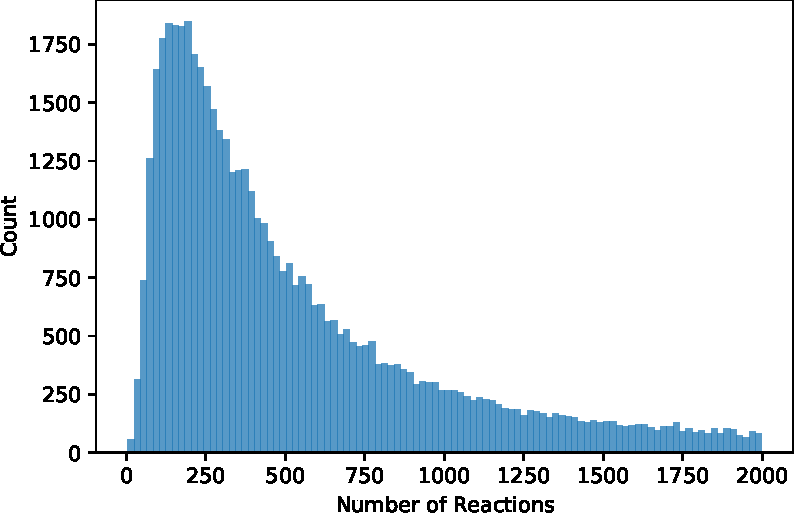
\includegraphics[width=.30\textwidth]{figures/dataset_rtnews/reactions_dist.pdf}
    \caption{rtnews Dataset}
    \label{fig:datasetstats-rtnews}
\end{figure} 
In contrast to the group dataset which consisted of heterogeneous posts made by a large
variety of users, the rtnews dataset only contained post of a single entity's Facebook 
page. Figure~\ref{fig:datasetstats-rtnews} gives some insights. The average message length
is longer. While the group dataset's most used post type was \emph{Photo} the most used type
for rtnews was \emph{Link}. As rtnews is a global television network, most of their posts
link to their own website. Most posts of the group dataset got no reactions at 
all. For rtnews the peak is about around 150 reactions per post.

\subsection{Dependent Variable}
We wanted to use this dataset to predict how much impact a post might achieve in a
specific group. A post has high impact if it gets more reactions as the average post of a 
group. We defined the set of posts for each Facebook group $G$ as follows
\[
    P_G = \{p_1, \dots, p_n\}
\]
with $p_1, \dots, p_n$ being individual posts. We can retrieve the sum of all kinds of
reactions that a specific post $p_i$ got by calling $r(p_i)$. First we calculated the average
number of reactions a post gets for each group  individually:
\[
    \tilde{p}_G = \frac{1}{n} \sum_{p_i \in P_G} r(p_i)
\]
The dependent variable we wanted to predict is a ratio of the post's reaction count and
the  average reaction count a post gets in a certain group $G$:
\[
    y(p_i) = \frac{r(p_i)}{\tilde{p}}
\]
For the rtnews dataset we assumed that we only have a single group and thus the dependent 
variable would only be the ratio of a post's reaction count and the average reaction count
inside rtnews.
%% - A post might get less attention if it goes down the timeline 
%%   => we only picked old posts
%% - picked a time range such that we get > 30,000 posts
%% - CT limitations max x posts...
%% \begin{itemize}
%%     \item Introduction to CrowdTangle
%%     \item Overview of our datasets (rtnews and conspiracy groups).
%%     \begin{itemize}
%%         \item How the data was collected
%%         \item Statistics/graphs explaining the datasets
%%     \end{itemize}
%%     \item Explanation of the conducted preprocessing
%%     \item Our score variable, description of the formula and the reasoning behind it
%% 
%%     \item Description of our task (i.e. predicting the impact of a post inside a group)
%%     \item Benefits which can be gained from this task (i.e. What triggers the success of 
%%     a post inside a certain group/echo chamber? How can one describe an usual post from a 
%%     certain group?)
%% \end{itemize}